% Chapter Template

\chapter{MODI} % Main chapter title

\label{Chapter5} % Change X to a consecutive number; for referencing this chapter elsewhere, use \ref{ChapterX}

\lhead{Capítulo 5. \emph{MODI}} % Change X to a consecutive number; this is for the header on each page - perhaps a shortened title

%----------------------------------------------------------------------------------------
%	SECTION 1
%----------------------------------------------------------------------------------------
\begin{figure}[htbp]
	\centering
		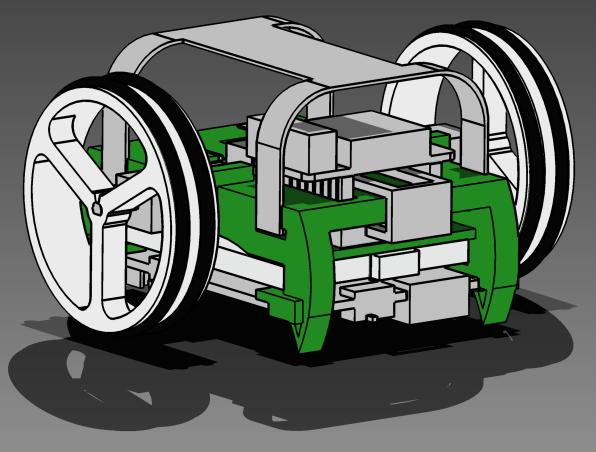
\includegraphics[width=0.8\textwidth]{./Figures/MODI/render.png}
	%	\rule{35em}{0.5pt}
	%\caption[Robot MODI]{robot MODI (sigla para Modular Intelligence)}
	\label{fig:MODI}
\end{figure}

Como se expuso en el capítulo anterior, actualmente existen varias alternativas de robots para comprar y construir un enjambre de robots. El problema es que o su precio es demasiado elevado o simplemente no son adaptables al tipo de investigación que se quiere realizar. Nuestro objetivo es tener un robot económico, fácil de reproducir y fabricable en la universidad para construir un enjambre de robots que permita hacer investigación y desarrollos en esta área.



\section{Diseño de Chasis MODI}
Luego de varias iteraciones (ver Figura \ref{fig:Historia})se logró el modelo final, ver Figura \ref{fig:compRender} b, que tiene cuatro piezas hechas en plástico PLA como se puede ver en la Figura \ref{fig:DiagramaVersionFinal}. 

Las piezas del robot fueron diseñadas para ser construidas por una máquina de prototipado rápido del tipo FDM, como una Reprap o MakerBot Replicator 2. Se debe tener en cuenta la tolerancia mecánica de las piezas. En especial hay dos piezas: la rueda y el chasis, que se unen al motor. Esta unión debe quedar con un ajuste mecánico Forzado Medio \footnote{http://campuscurico.utalca.cl/\~ fespinos/Ajustes\%20y\%20tolerancias\%20mecanicas.pdf}, para que estas uniones queden fijas y las ruedas estén en el eje correspondiente.

Está formado por cuatro partes:

\begin{enumerate}
\item Chasis, que es la pieza que une a todos los componentes y cumple con el \textbf{Requerimiento 4}. Ver Figura \ref{fig:Render Piezas 3D} a.
\item Ruedas, permiten el desplazamiento y poseen dos canales para poner o-ring y así aumentar el roce con la supercifie. Ver Figura \ref{fig:Render Piezas 3D} d.
\item Accesorio, tiene un sistema de anclaje al chasis que permite tener distintas carcasas y sensores. Ver Figura \ref{fig:Render Piezas 3D} b.
\item Logo,  sujeta parte de la electrónica contenida en el Chasis y dos LEDs RGB. Ver Figura \ref{fig:Render Piezas 3D} c.
\end{enumerate}

Cada una de estas piezas puede ser vista en la Figura \ref{fig:Render Piezas 3D}.

Usando una Replicator 1 de MakerBot, la pieza que más demora en construirse es el Chasis, que son 108 minutos. Cada Rueda demora 20 minutos, el accesorio 58 minutos y el logo 25 minutos. Se resume en la Figura

\begin{figure}[htbp]
	\centering
		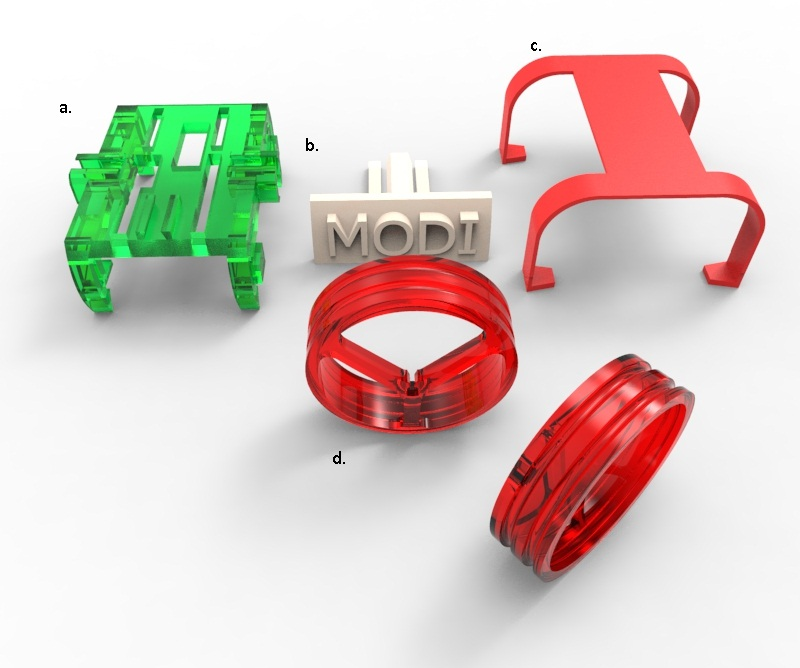
\includegraphics[width=\textwidth]{./Figures/MODI/piezas.jpg}
		\rule{35em}{0.5pt}
	\caption[Piezas 3D]{Las cinco piezas que componen el hardware mecánico de MODI, estas son: a) el chasis, d) las dos ruedas, c) el accesorio y b)logo. Las dimensiones del robot MODI ensamblado son 96[mm] de diámetro y 50 [mm] de alto.}
	\label{fig:Render Piezas 3D}
\end{figure}

\begin{figure}[htbp]
	\centering
		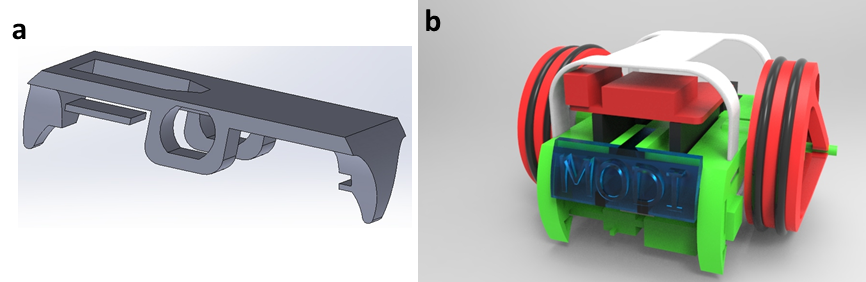
\includegraphics[width=\textwidth]{./Figures/MODI/compRender.png}
		\rule{35em}{0.5pt}
	\caption[Comparación entre el primer render realizado y el último]{\textbf{ a.} Primer Chasis de MODI, realizado con SolidWorks 2012. Esta versión sirve sólo como prueba de concepto ya que no tiene espacio para las conexiones eléctricas necesarias.\textbf{ b.} Última versión de MODI a la fecha, el diseño se realizó en Inventor 2013 y el render se obtuvo con KeyShot 4.}
	\label{fig:compRender}
\end{figure}	

\begin{figure}[htbp]
	\centering
		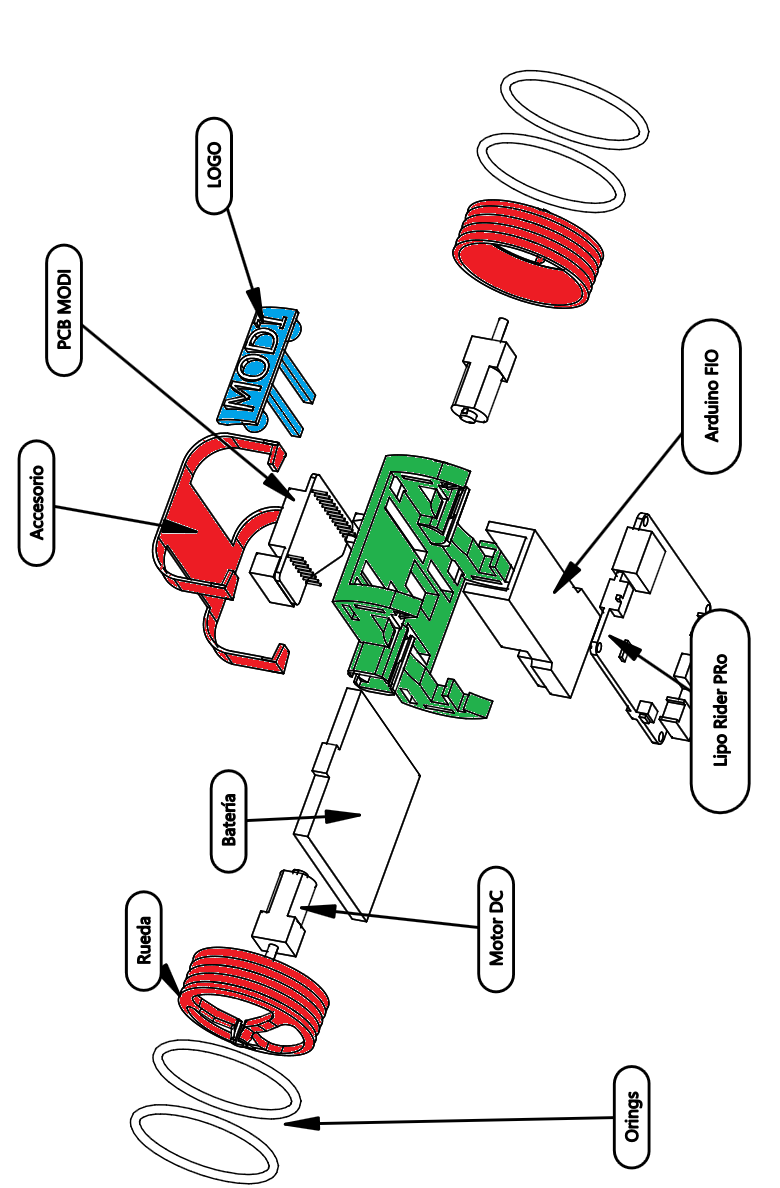
\includegraphics[width=\textwidth]{./Figures/MODI/ensamble.png}
		\rule{35em}{0.5pt}
	\caption[Diagrama MODI versión final]{Diagrama de todos los componentes que forman parte de MODI, este diagrama sirve de guía para poder ensamblarlo.}
	\label{fig:DiagramaVersionFinal}
\end{figure}	

\FloatBarrier
%-----------------------------------
%	SUBSECTION 5
%-----------------------------------
\section{Diseño de PCB MODI}

En los primeros prototipos un problema que se repetía constantemente fueron las conexiones entre los sistemas que componen al robot. Son 15 conexiones que unen distintos componentes, Figura \ref{fig:Diagrama cables}. Por esto se requiere un PCB que permita reducir al mínimo el espacio necesario para energizar y comunicar los componentes. El requerimiento principal es poder fabricarlo con una fresa CNC como la Roland Modela MDX-20, por lo que para facilitar el proceso de construcción es necesario diseñar un PCB de una sola capa. Se utilizó Eagle como software para el diseño del diagrama eléctrico y PCB, el resultado se puede ver en la Figura \ref{fig:pcb}.


\begin{figure}[htbp]
	\centering
		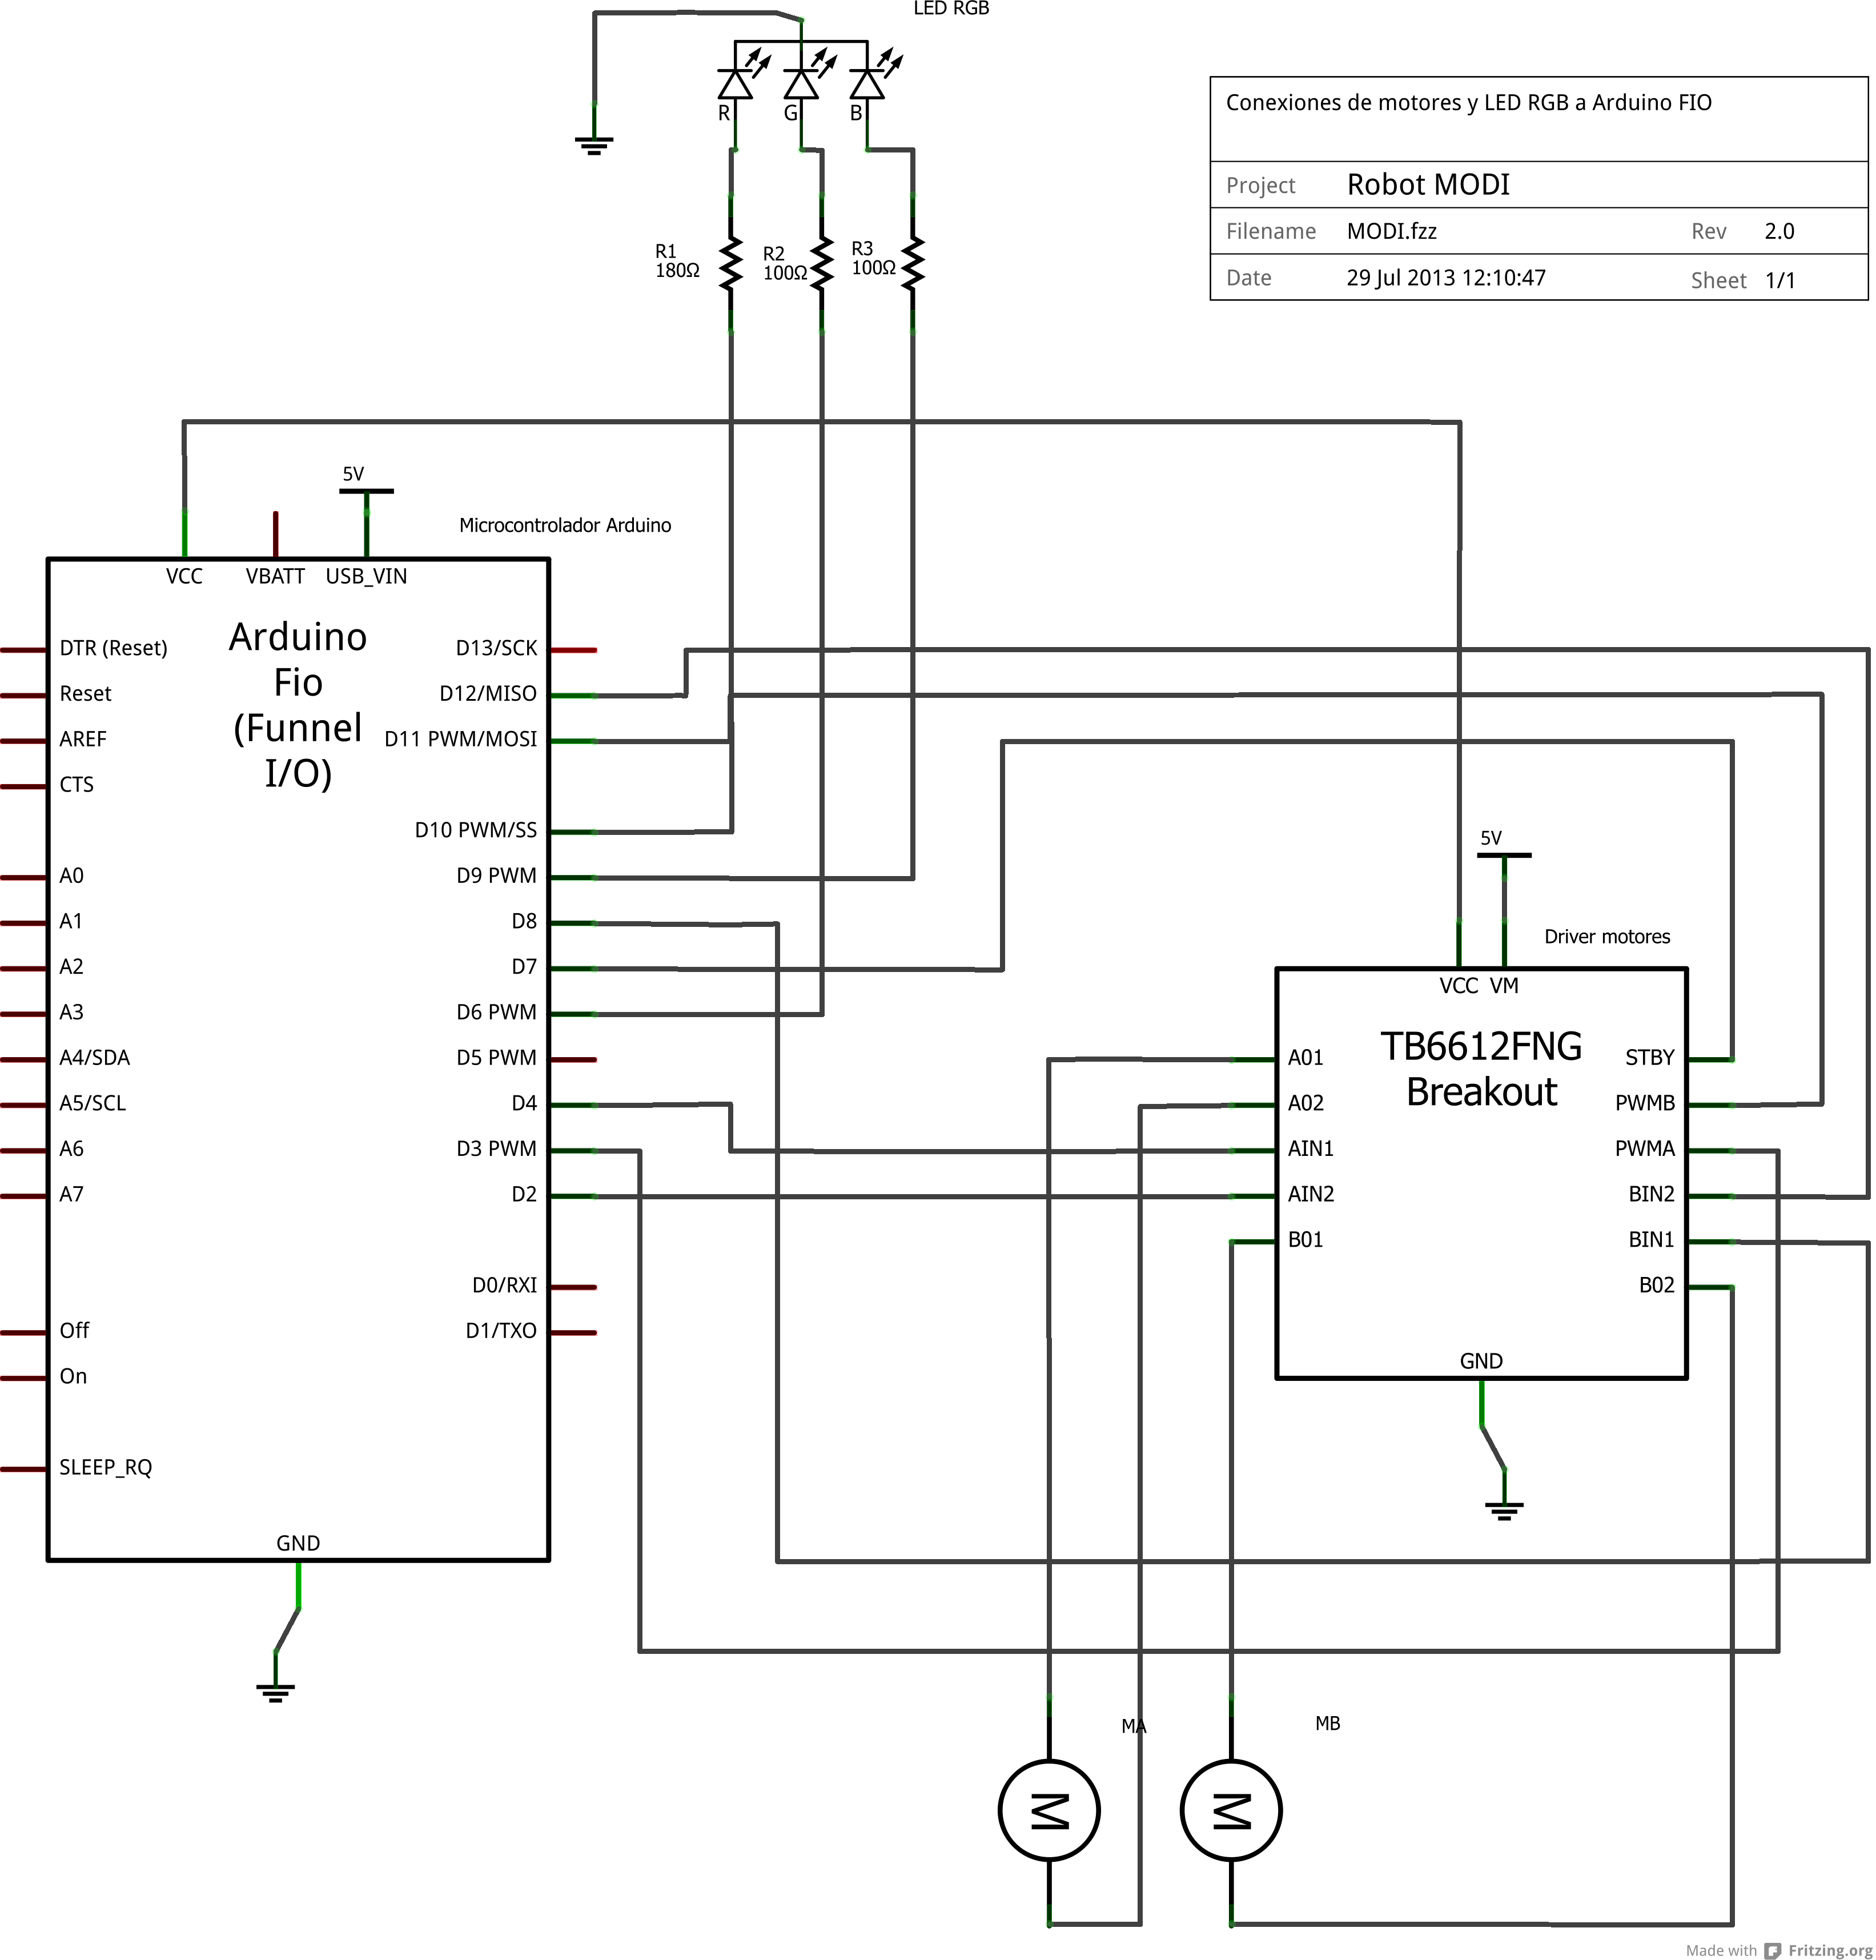
\includegraphics[width=\textwidth]{./Figures/modi/MODI_schem.png}
		\rule{35em}{0.5pt}
	\caption[Diagrama eléctrico de conexiones en PCB MODI]{Diagrama de conexiones eléctricas en PCB diseñada para MODI. Está realizado en Fritzing.2013.07.27.pc.}
	\label{fig:Diagrama cables}
\end{figure}	

\begin{figure}[htbp]
	\centering
		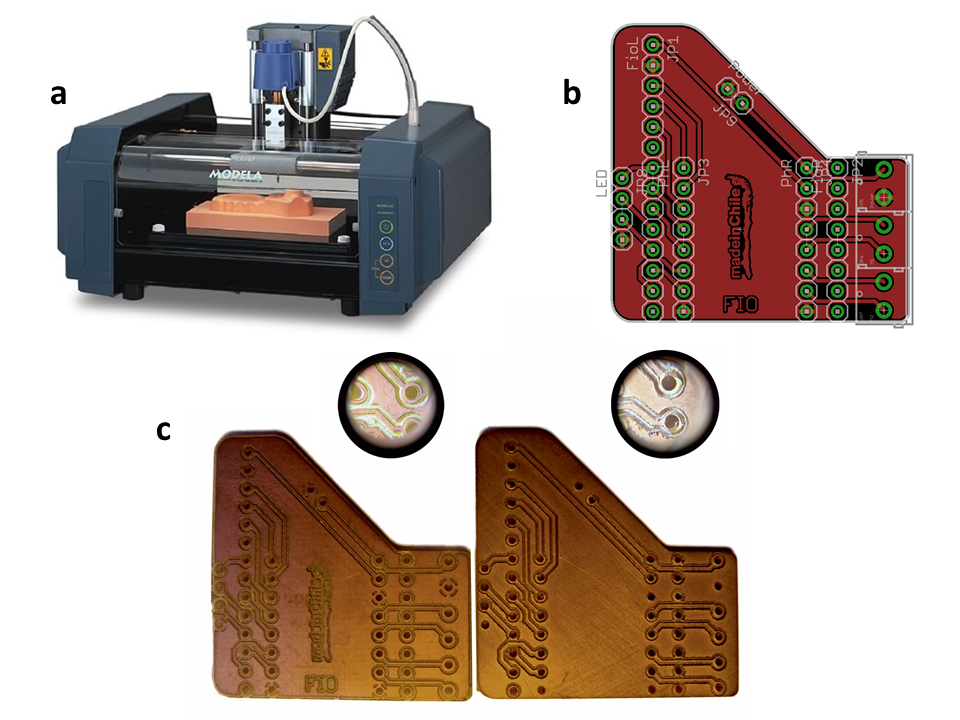
\includegraphics[width=0.9\textwidth]{./Figures/modi/pcb.png}
		\rule{35em}{0.5pt}
	\caption[Fabricación de PCB]{\textbf{a.} Roland Modelo MDX-20 usada para hacer PCB y modelos 3D \textbf{b.} MODIBoard es una PCB diseñada para poder conectar de forma simple los diversos componentes electrónicos. Conecta: Arduino Fio, Lipo Rider Pro, Motor Driver, LED RGB y Motores, \textbf{c. }PCB fresada en dos máquinas diferentes. Se puede apreciar en el detalle aumentado 60x, la importancia de contar con una buena resolución de fresado. En especial es necesario tener un buen pad para facilitar el soldado.}
	\label{fig:pcb}
\end{figure}

%-----------------------------------
%	SECTION 2
%-----------------------------------

\section{Componentes electrónicos}

\begin{figure}[htbp]
	\centering
		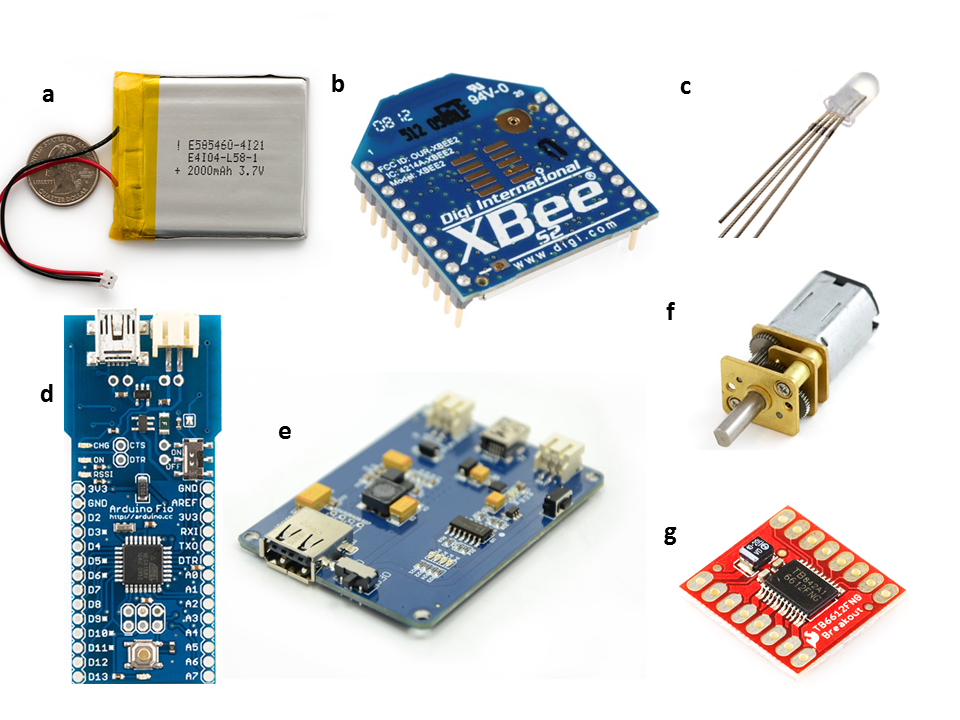
\includegraphics[width=\textwidth]{./Figures/MODI/compElo.png}
		\rule{35em}{0.5pt}
	\caption[Componentes Electrónicos]{Todos los componentes electrónicos que forman MODI \textbf{ a.} Batería LIPO 2,000 mAh, \textbf{b.} XBee, \textbf{c.} LED Rgb difuso, de esta manera se obtiene un ángulo de visión mucho más amplio, \textbf{d.} Arduino Fio, \textbf{e.} Lipo Rider Pro,\textbf{ f.} Motor DC 30:1 \textbf{g.} Motor Driver 1A Dual TB6612FNG.}
	\label{fig:compELO}
\end{figure}

MODI está compuesto por varios componentes electrónicos que implementan tecnologías nuevas. De forma sencilla el usuario puede hacer uso de todas estas, que por ser Open Source tienen una amplia documentación. Su uso en colegios, talleres y universidades, por ser de bajo costo, y sin partes externas extremadamente frágiles, es una excelente herramienta para iniciar a alumnos en temas como la Programación, Robótica, Comunicación Inalámbrica y Visión Artificial, entre otros, sin los miedos asociados a utilizar un equipo costoso y delicado.

El robot MODI es pequeño y de fácil construcción con las herramientas de Fabricación Digital que se pueden encontrar en un FabLab. Tiene un pequeño microcontrolador \textbf{Arduino} que controla dos motores, y un \textbf{XBee} para la comunicación inalámbrica con un computador central que usando cualquier lenguaje de programación con comunicación serial puede controlar uno o más robots. La posición de cada robot se obtiene con tags \textbf{Fiduciales}, que permiten por medio de una cámara cenital saber la coordenada y rotación de cada uno. En esta primera aplicación es necesario contar con autonomía energética por lo que se incluye una batería lipo de 2000[mAh] junto a un módulo que carga la batería y eleva el voltaje de salida a 5[v]. Este módulo de carga, \textbf{Lipo Rider Pro}, tiene además la ventaja de permitir distintos tipos de carga, como una celda de carga solar o un sistema de carga inalámbrica por medio de bobinas. Tener la posibilidad de cargar una batería con luz solar o por medio de forma inalámbrica hace posible el hacer experimentos que necesiten estar funcionando semanas sin la intervención de un humano para cargar cada uno.

A continuación describiremos en detalle cada uno de los componentes utilizados en MODI. Las especificaciones técnicas de cada uno de ellos se encuentra resumida en la tabla \ref{fig:TablaElo}

%-----------------------------------
%	SUBSECTION 1
%-----------------------------------
\subsection{Arduino FIO}
El Arduino FIO, Figura \ref{fig:compELO} d, ha sido diseñado por Shigeru Kobayashi, es una placa para microcontrolador basada en el ATmega328P. Funciona a 3.3V y 8 MHz. Tiene 14 pines de I/O digitales (de los cuales 6 pueden usarse como salidas PWM), 8 entradas analógicas, un oscilador en placa, un botón de reinicio (reset), y agujeros para montar conectores de pines. Tiene conexiones para una batería de polímero de Litio e incluye un circuito de carga a través de USB. En el reverso de la placa tiene disponible un zócalo para módulos XBee.

El Arduino FIO está diseñado para aplicaciones inalámbricas. El usuario puede subir sus sketches con un cable FTDI o una placa adicional adaptadora Sparkfun. Además, si utiliza un adaptador de USB a XBee modificado (como el USB Explorador de XBee), el usuario puede subir sketches de forma inalámbrica. La tarjeta viene sin conectores pre-montados, permitiendo el uso de diversos tipos de conectores o la soldadura directa de los cables. 

%-----------------------------------
%	SUBSECTION 2
%-----------------------------------
\subsection{Motores DC}
Para MODI se utilizan motores DC de la marca Pololu, Figura \ref{fig:compELO} f. Este motor se caracteriza por su reducido tamaño (largo: 9.27 mm), por lo que los motores usan muy poca corriente y constan con una caja de reducción metálica de 30:1. El eje tiene forma de D, lo que permite una unión firme entre el motor y la rueda de plástico, evitando deslizamientos.

Pese a no ser la alternativa más económica, estos motores han sido muy difundidos para su uso en robótica por su bajo consumo y alto torque. 
%-----------------------------------
%	SUBSECTION 3
%-----------------------------------
\subsection{XBee}

Los dispositivos con los cuales interactuamos a diario poseen acceso a distintos tipos de sistemas de comunicación. Los \textit{Smartphone} cuentan con diversas antenas para conectarse a WIFI, Bluetooth, red celular,  por nombrar algunas. Estamos en un momento en que las comunicaciones son una de las claves tecnológicas que nos permiten cumplir con tareas que hace algunos años eran imposibles de hacer en un día. Es claro que un sistema con varios o cientos de robots también necesitan comunicarse. Y en el caso particular de MODI, que por el momento no tiene sensores, es fundamental la información que se transmita para controlarlo. 

Para comunicar un robot con otro pueden usarse diversas técnicas. Dependiendo del área en particular que sea del interés del científico, los robots pueden comunicarse por medio de sensores de proximidad o tacto. Para saber que hay otro cerca, pueden tener un sistema de visión artificial con una cámara a bordo que le permita “ver” el entorno al robot, con parlantes y micrófonos pueden emitir algún ruido que sea interpretado por su entorno, o lo mismo con sensores de otros tipos.

En nuestro caso optamos por usar el protocolo ZigBee, y para esto hacemos uso de los dispositivos XBee de la empresa Digi. Existen varios modelos de XBee con distintos tipos de antena (chip, alambre o conector SMA), potencia de transición (2mW - 60mW) y frecuencia de operación (2.4 GHz y 900 MHz). Además son de bajo consumo (50mA en funcionamiento) y se puede tener una gran distancia de comunicación (1.6 Km). Otra característica importante de los XBee es que son capaces de formar redes MESH, que es un tipo de red donde los dispositivos se pueden agregar o remover en forma dinámica y los dispositivos pueden ayudar a dispositivos fuera de alcance a  conectarse con el computador principal. Como el proyecto está diseñado para funcionar dentro de un laboratorio pequeño se escogió el XBee Serie 2 de 2mW con antena chip, ya que son los más económicos por ser para comunicación a corta distancia. Con esto se cumple con el \textbf{Requerimiento 9}.

%-----------------------------------
%	SUBSECTION 3
%-----------------------------------
\subsection{Lipo Rider Pro}
 La versión actual de MODI permite su carga por medio de un puerto Mini USB, panel solar y de forma inalámbrica. cumpliendo con el \textbf{Requerimiento 5}.

El LiPo Rider Pro, Figura \ref{fig:compELO} a, es una versión mejorada del LiPo Rider, que es una fuente de poder para alimentar distintos gadget con energía solar. Esta placa permite alimentar con 5V distintos dispositivos. Cuya energía puede provenir de diferentes fuentes, tales como, energía del sol o por medio de inducción magnética y almacena esta energía en una batería LiPo. Esta PCB es extremadamente útil ya que además de energizar a MODI, puede incluso cargar un SmartPhone para poder más adelante extender las capacidades de procesamiento del robot.

La Lipo Rider obtiene de dos formas la energía, una es con un panel solar y la otra es directamente con un puerto mini USB. Con esta energía carga una batería de Litio Polímero de 3.7V. Como salida entrega 5V a 1A. Además tiene un botón con 4 LEDS que indican el estado de carga de la batería.

%-----------------------------------
%	SUBSECTION 4
%-----------------------------------
\subsection{Motor Driver 1A Dual TB6612FNG}
El TB6612FNG motor driver puede controlar hasta dos motores DC, a una corriente constante de 1.2A (3.2A peak) y así separar la lógica del Arduino con la potencia que necesitan los motores. Dos señales de entrada (IN1 y IN2) puede ser usadas para controlar el motor en una de cuatro modos de funcionamiento: giro horario, giro anti horario, short-brake, y parada. A cada motor se le conectan dos salidas y cada motor se puede controlar separadamente, la velocidad de cada uno es controlada vía pin PWM y puede alcanzar las 440 RPM. El pin STBY debe colocarse en High para que el motor salga del estado Standby. Ver Figura  \ref{fig:TB6612FNG} para las conexiones. Con esto se cumple el \textbf{Requerimiento 8}.

\begin{figure}[htbp]
	\centering
		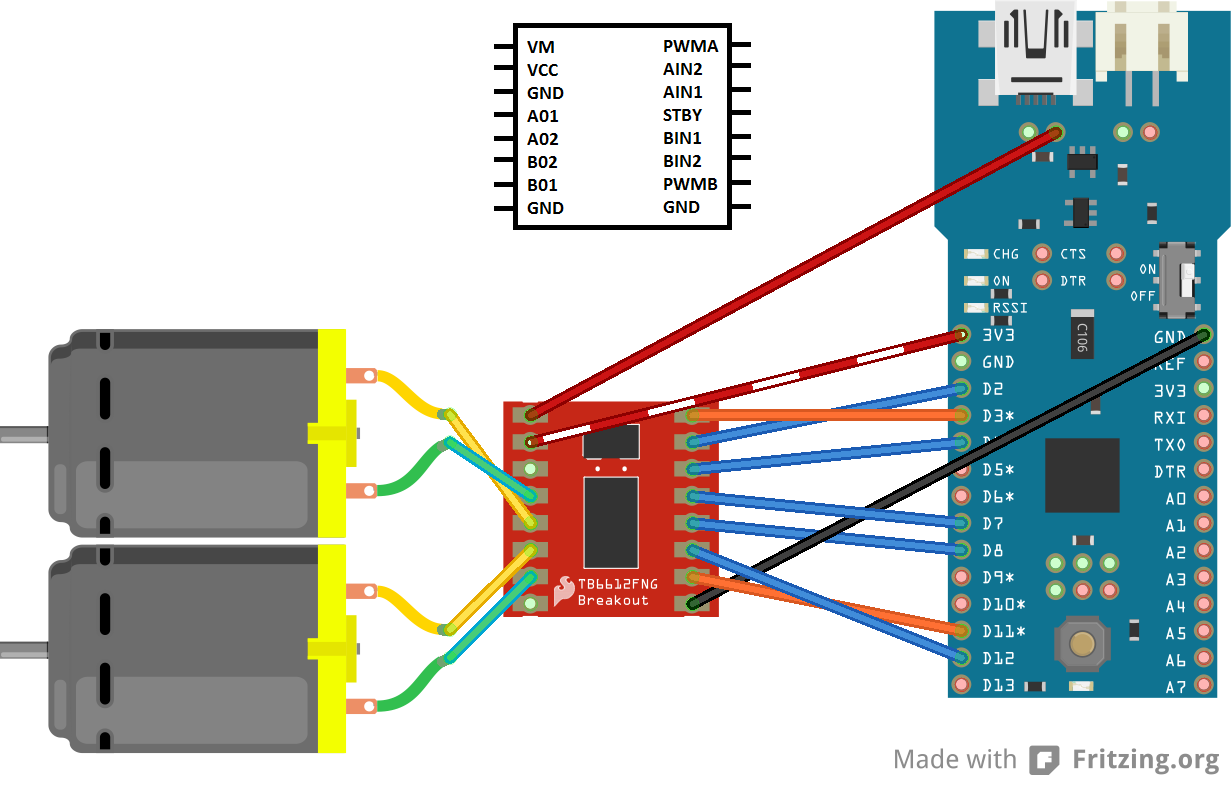
\includegraphics[width=0.8\textwidth]{./Figures/MODI/MODI_without_LED_bb.png}
		\rule{35em}{0.5pt}
	\caption[Conexión eléctrica Motor Driver 1A Dual TB6612FNG]{Diagrama de conexiones eléctricas para conectar Motor Driver 1A Dual TB6612FNG con motores DC y Arduino FIO.}
	\label{fig:TB6612FNG}
\end{figure}

%\FloatBarrier

%-----------------------------------
%	SUBSECTION 3
%-----------------------------------
\subsection{Batería LiPo y LED RGB}

Al comienzo se utilizaron baterías AAA para el robot, pero estas tienen el problema de que es necesario que el usuario las retire del robot para recargarlas. Por su parte las baterías LiPo permiten cargarse con el circuito de la Lipo Rider Pro y posee una alta densidad de carga, 2000mAh a 3.7V, que significa casi 3 horas de autonomía en funcionamiento continuo de los motores. Esta batería ayuda a cumplir con el \textbf{Requerimiento 5.}

El \textbf{Requerimiento 7} se cumple incluyendo un LED RGB, que se puede controlar de manera simple para indicar los distintos estados en que puede encontrarse el robot. En la Figura \ref{fig:LED} se puede ver un diagrama de conexiones.

\begin{figure}[htbp]
	\centering
		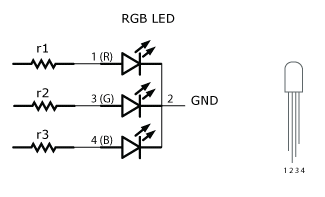
\includegraphics[width=0.8\textwidth]{./Figures/MODI/RGBLED.png}
		\rule{35em}{0.5pt}
	\caption[Conexión eléctrica LED RGB]{Diagrama de conexiones eléctricas para LED RGB. Para obtener un brillo óptimo se recomienda usar los valores de resistencias: 180 Ohm Rojo, 100 Ohm Verde, 100 Ohm Azul.}
	\label{fig:LED}
\end{figure}

\begin{figure}[htbp]
	\centering
		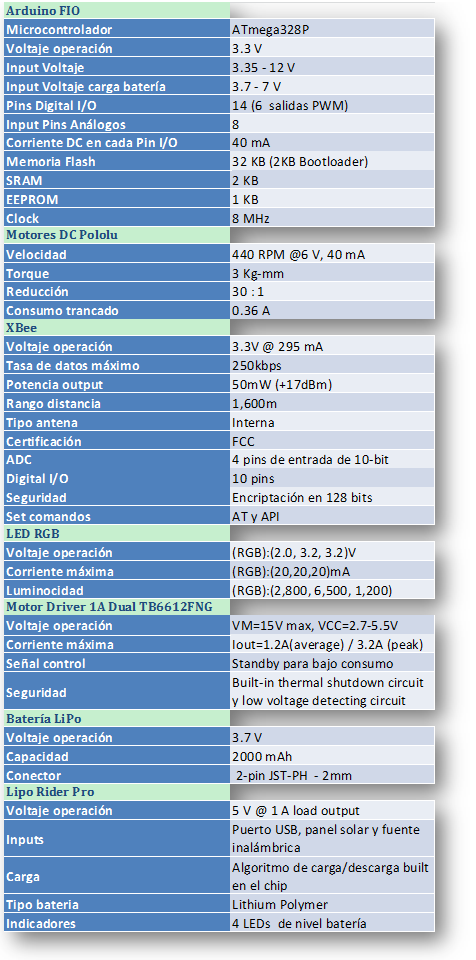
\includegraphics[width=0.8\textwidth]{./Figures/MODI/comparacionElo.png}
		\rule{35em}{0.5pt}
	\caption[Tabla caracteristicas más importantes de los componentes Eléctronicos]{Resumen de las características más importantes de los componentes electrónicos que tiene MODI.}
	\label{fig:TablaElo}
\end{figure}


%-----------------------------------
%	SECTION 4
%-----------------------------------

\section{Locomoción}
Existen distintas áreas donde se utilizan robots, dependiendo de la tarea a realizar es la movilidad que éste debe tener. Algunos tienen complejos sistemas como la plataforma del proyecto Atlas (The Agile Anthropomorphic Robot) de Boston Dynamics, Figura \ref{fig:Atlas}. En nuestro caso, sólo es necesario desplazarse sobre una superficie plana y por esto, en vez de tener costosos actuadores neumáticos, la solución más simple es contar con dos motores para poder tener un movimiento diferencial. Si se desea tener más información sobre los tipos de locomoción en robots con ruedas, ver esta pagina web\footnote{en.wikibooks.org/wiki/Robotics/Types\_of\_Robots/Wheeled}.


\begin{figure}[htbp]
	\centering
		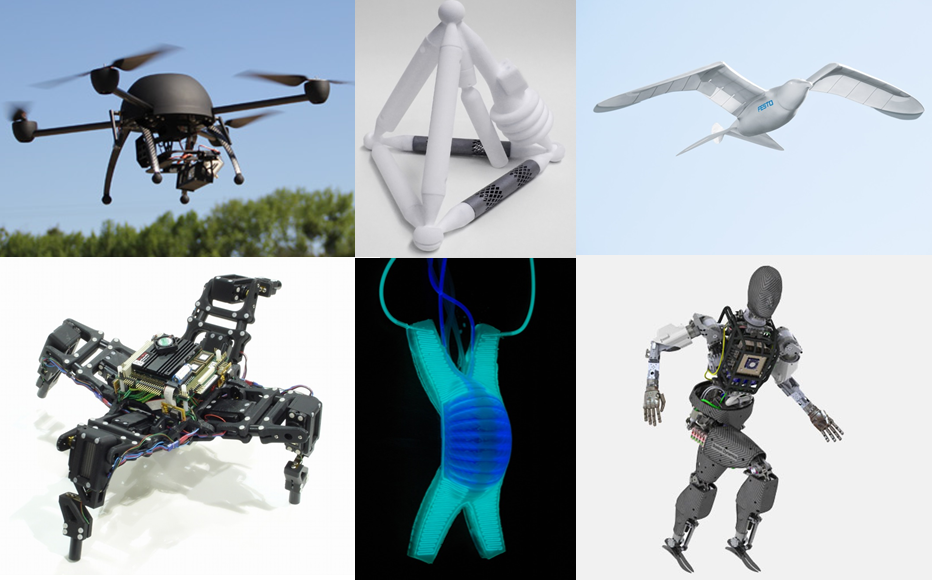
\includegraphics[width=\textwidth]{./Figures/robots.png}
		\rule{35em}{0.5pt}
	\caption[Robots]{Varios robots con distintos tipos de locomoción.}
	\label{fig:Atlas}
\end{figure}


Para moverse MODI tiene dos motores DC, ver Figura \ref{fig:compELO} f. Estos tienen una caja de reducción 30:1 que permiten aumentar el torque hasta 3 Kg-mm y disminuir la velocidad máxima hasta las 440 RPM. La Figura \ref{fig:DCMotor} a, muestra como se relaciona la velocidad y el consumo de corriente con el torque del motor.

\begin{figure}[htbp]
	\centering
		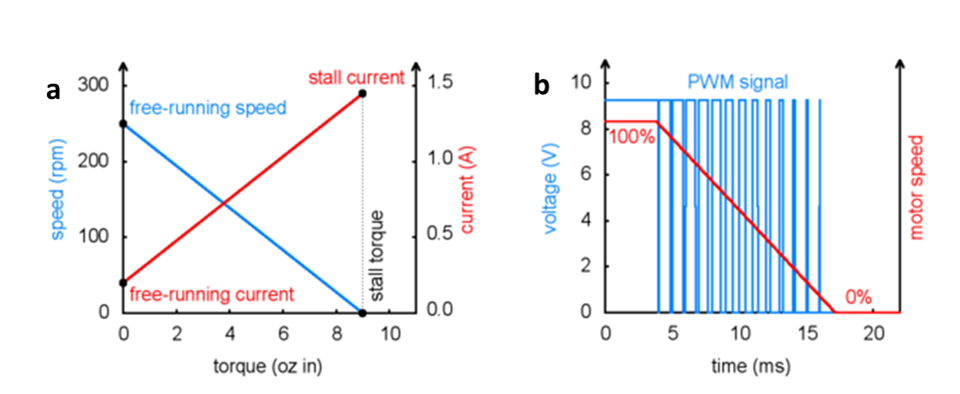
\includegraphics[width=0.8\textwidth]{./Figures/graficosMotores.png}
		\rule{35em}{0.5pt}
	\caption[Gráficos Motor DC]{a. Operación motores: Corriente, velocidad y torque. Imagen extraída de pololu.com, b. Control de velocidad PWM, se observa como disminuye la velocidad según ciclo de trabajo.}
	\label{fig:DCMotor}
\end{figure}

El control de velocidad de los motores se hace por medio de una señal PWM que se genera en el arduino. La señal PWM es periódica y se modifica solo su ciclo de trabajo, ver Figura \ref{fig:pwm}, que está relacionado con el valor medio de la señal. De manera que con una señal PWM con un ciclo de trabajo menor se obtiene un voltaje de salida menor, por ende una menor velocidad en el motor.  La Figura \ref{fig:DCMotor} b, relaciona el valor de la señal PWM como un voltaje con la velocidad del motor. Esta es una forma práctica de obtener salidas análogas desde una salida digital en Arduino. 
La potencia de los motores es controlada con el chip TB6612FNG, ver Figura \ref{fig:TB6612FNG}. En este diagrama se pueden ver dos cables naranjos, que son los que controlan la velocidad. En el Arduino se generan señales PWM en sus pins D3 y D11. Los valores que genera el Arduino para control de velocidad de los motores como representación interna de la señal PWM van desde 0 a 255, y además se puede controlar el sentido de giro según las salidas AIN y BIN. Por ejemplo para hacer que la rueda izquierda gire en sentido horario se debe dejar el pin AIN1 en 0 y AIN2 en 1 y la velocidad de ésta va a ser según el valor de la señal en PWMA, ver Figura \ref{fig:pwm} b. Para los distintos casos se puede ver la Figura \ref{fig:pwm} a, que indica los 3 movimientos que son: avanzar, avanzar hacia a la izquierda y girar en el eje. Aquí los números representan el período del ciclo de trabajo de la señal enviada por el Arduino al controlador de los motores. 

Se puede realizar un control más fino de la posición usando la información de posición del robot con un Control Proporcional, Integral y Diferencial (PID). El PID es para controlar un sistema realimentado, donde se calcula la desviación (error) entre un valor medido (la posición obtenida con el sistema de tracking) y el valor que se quiere obtener, para aplicar una acción correctora que ajuste el proceso. En este algoritmo hay tres parámetros distintos: el proporcional, el integral y el derivativo. El valor del parámetro proporcional produce una señal proporcional a la desviación de la salida del proceso. El integral elimina el problema del error en estado estacionario frente a perturbaciones de carga constante y el derivativo determina la reacción según el tiempo donde el error se produce. Estos tres parámetros permiten controlar la posición y/o orientación del robot MODI. Se recomienda ver este vídeo tutorial \footnote{http://www.youtube.com/watch?v=aE7RQNhwnPQ}. 

\begin{figure}[htbp]
	\centering
		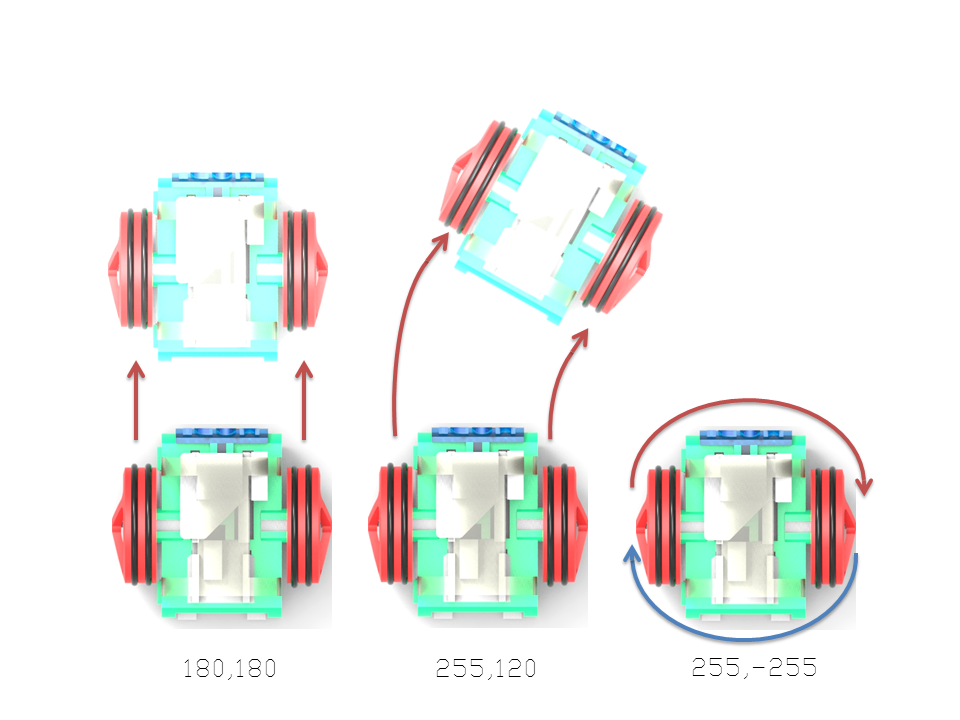
\includegraphics[width=\textwidth]{./Figures/MODI/pwm.png}
		\rule{35em}{0.5pt}
	\caption[Señal PWM]{Movimiento diferencial. A diferencia de un auto, MODI tiene dos motores que giran de forma independiente. Las distintas velocidades y sentido de giro determinan el ángulo para girar. Si se necesita solamente rotar los motores deben girar en sentidos opuestos. Se utiliza -255 en la última Figura para referirse a una señal PWM de 255 pero con sentido contrario.}
	\label{fig:pwm}
\end{figure}

%-----------------------------------
%	SECTION 5
%-----------------------------------
\section{Implementación}
La construcción de MODI fue motivada por una aplicación concreta, que es tener un grupo de robots controlables de forma independiente para hacer estudios del comportamiento del grupo. Para esto fue necesario montar un sistema simple con una cámara cenital que vigila  la posición y orientación de cada uno de ellos.

El robot que se construyó para hacer las pruebas cuenta con un sistema externo de visión artificial que permite obtener posición y orientación de cada robot. Esto es necesario ya que como se mencionó, no existe ningún sensor interno del robot que le pueda ayudar a ubicarse en el espacio. Esta información es transmitida a cada robot por medio del protocolo \textit{zigbee} implementado en los chip XBee de la empresa Digi, ver Figura \ref{fig:compELO} b. Esto permite comunicar un alto número de robots, con muy poco consumo energético y de manera relativamente simple. Se escogió usar visión artificial sobre el sistema para bajar los costos individuales de los robots y XBee por ser el estándar en la industria en redes de sensores inalámbricos. Cabe destacar que los robots que existen en el mercado no incluyen XBee, y los que lo traen lo hacen como accesorio. 
%-----------------------------------
%	SECTION 6
%-----------------------------------

\subsection{Setup}

Para investigar el comportamiento colectivo de un grupo de robots, en el mundo real sin hacer uso de simuladores, es necesario contar con un lugar físico donde poder activar los robots. Además para simplificar cada uno de los robots, estos no tienen sensores internos por lo que hay una cámara montada sobre el plano de movimiento de estos, para hacer Seguimiento Visual. Esta información de coordenadas llega a un computador servidor que le indica a cada robot cómo moverse.
\begin{figure}[htbp]
	\centering
		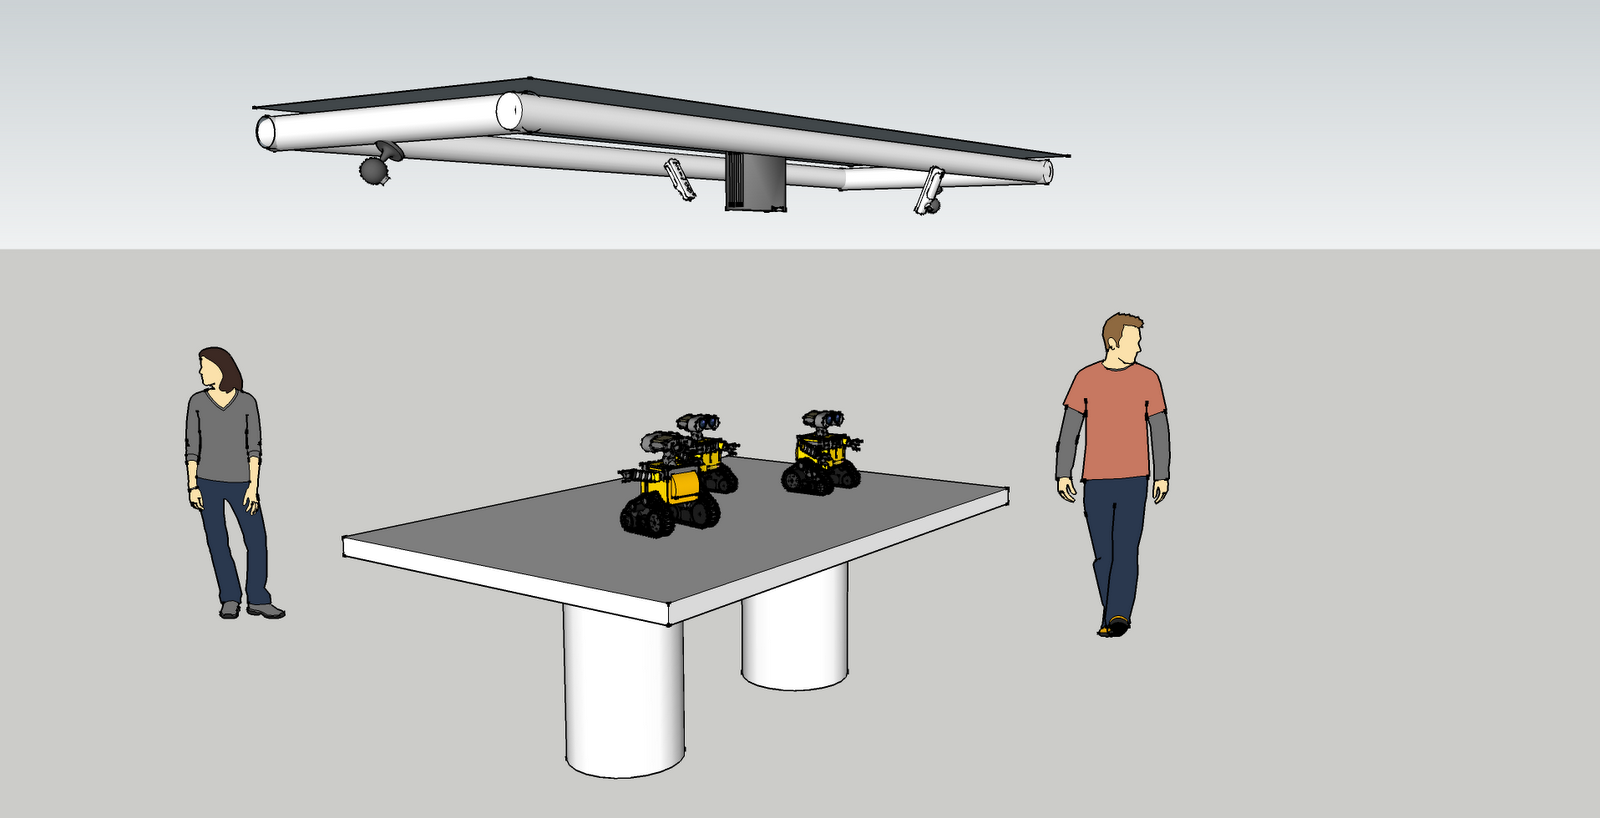
\includegraphics[width=\textwidth]{./Figures/setup.png}
		\rule{35em}{0.5pt}
	\caption[Setup Enjambre MODI]{Setup a montarse para hacer estudios de grupos de robots.}
	\label{fig:setup}
\end{figure}
%-----------------------------------
%	SUBSECTION 6
%-----------------------------------

\subsection{Software}

El software de MODI es bastante sencillo. Básicamente se configuraron todas las variables para cumplir con las conexiones eléctricas definidas en la Figura \ref{fig:Diagrama cables} y un puerto serial que está a la espera de comandos que indican acciones del robot. El puerto serie en MODI se configuró a una velocidad de 115200 y está esperando los caracteres ‘w’,’a’,’d’ y ‘s’, como Adelante, Izquierda, Derecha y Atrás respectivamente. 

Firmware y algunos ejemplos para testear funciones de manera individual se encuentran en el Git de MODI en Github. \footnote{https://github.com/FabLabUChile/modi}


\subsection{Tracking 2D}
Al igual que los seres vivos un robot necesita \textit{sentidos} o algún sistema sensorial para poder interactuar con su entorno. Estos pueden ser sensores IR para detectar objetos cercanos, cámaras o LASER para hacer un mapa del entorno o simplemente un pulsador que sea presionado cada vez que el robot colisiona. Para bajar costos, MODI actualmente no cuenta con sensores “onBoard”. Cada robot es comandado por un sistema que le dice donde está él, donde están los demás, y los límites del área de trabajo. Se diseñó de esta manera para simplificar la programación de cada robot.

reacTIVision \cite{kaltenbrunner2007reactivision} es un framework Open Source, cross-platform, para realizar tracking rápido y robusto de tags fiduciales, pegadas a objetos físicos, ver Figura \ref{fig:Fiducial}. Ha sido diseñado como un toolkit para el desarrollo rápido de multi-touch interactive surfaces. Este framework fue desarrollado por Martin Kaltenbrunner y Ross Bencina en el Music Technology Group de la universidad de Pompeu Fabra en Barcelona, España. reacTIVision fue diseñado como sensor principal de la Reactable, un sintetizador modular tangible que ha marcado los standards en lo que a aplicaciones multitouch se refiere. 
Esta alternativa debe ir acompañada de otros elementos, como la cámara y el computador en el cual se ejecuta el software. Con estos elementos mediante un protocolo llamado TUIO, disponible como biblioteca en los lenguajes de programación más populares, se puede obtener: la posición, orientación e identificador de cada robot, cumpliendo con el \textbf{Requerimiento 6}. Con reacTIVision es posible detectar hasta 216 tag fiduciales a una velocidad de 50 fps a una resolución de 640 x 480.




\begin{figure}[htbp]
	\centering
		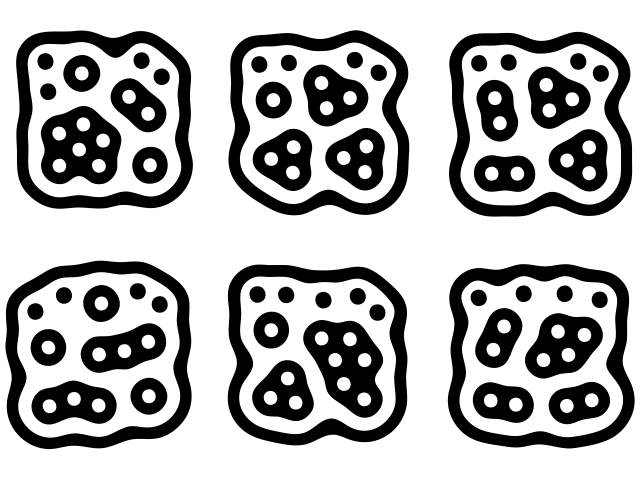
\includegraphics[width=0.65\textwidth]{./Figures/MODI/fiducial.png}
		\rule{35em}{0.5pt}
	\caption[Fiduciales usados como tag en reacTIVision]{Códigos fiduciales utilizados en reacTIVision. Estos códigos aunque parecen algo extraños para los seres humanos están diseñados de tal forma que es muy fácil diferenciar unos de otros y además obtener su orientación y posición en un software de análisis de imágenes. Se tiene un total de 216 configuraciones posibles de códigos.}
	\label{fig:Fiducial}
\end{figure}



%-----------------------------------
%	SECTION 7
%-----------------------------------

\subsection{Bill Of Material}

Con un precio total de 180 USD, Figura \ref{fig:BOM}, MODI se propone como una alternativa económica para construir un robot de desplazamiento diferencial. Pensando en comprar desde Chile, son tres las tiendas en que se cotizaron los componentes. Es posible comprar todo desde internet. Para más detalles sobre la Lista de materiales ver link \footnote{http://kitbom.com/otrab/modi}.
\begin{figure}[htbp]
	\centering
		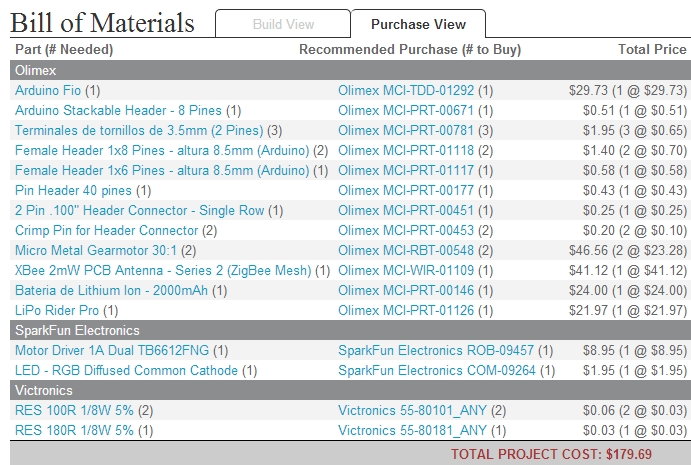
\includegraphics[width=\textwidth]{./Figures/MODI/kitbom.png}
		\rule{35em}{0.5pt}
	\caption[Bill Of Materials]{Lista de materiales a comprar para construir un robot MODI, la versión online de este BOM se puede ver en http://kitbom.com/otrab/modi}
	\label{fig:BOM}
\end{figure}

Luego de haber seleccionado los componentes se incluye la tabla en la Figura \ref{fig:Tabla robots MODI} que compara al robot MODI con los otros robots estudiados en el capítulo 3.

\begin{figure}[htbp]
	\centering
		\includegraphics[width=0.6\textwidth]{./Figures/tabla_robots_modi.png}
		\rule{35em}{0.5pt}
	\caption[Tabla comparativa robots MODI]{En esta tabla se comparan las características principales del robot MODI con los robots: kilobot, e-puck y 3pi.}
	\label{fig:Tabla robots MODI}
\end{figure}
